\documentclass[xcolor=pdftex,dvipsnames,table,mathserif]{beamer}
%\usepackage{subfigure}
\usepackage{amsbsy}
\usepackage{tikz}
\usetikzlibrary{arrows}
\usepackage{amsmath,graphicx,dsfont,color}
\usepackage{amsfonts}
\usepackage{amssymb}
\usepackage{array}

\usepackage{subfig}

% makes the subfig package work
\makeatletter
\let\@@magyar@captionfix\relax
\makeatother

% subfigure counter resets every frame
\makeatletter
\@addtoreset{subfigure}{framenumber}
\makeatother

% First author and year
\bibliographystyle{apalike}

% This sets the list items of the bibliography to the same symbol used for citation.
\setbeamertemplate{bibliography item}{\insertbiblabel}

% This avoids extralines for different entries
\setbeamertemplate{bibliography entry title}{}
\setbeamertemplate{bibliography entry location}{}
\setbeamertemplate{bibliography entry note}{}

\DeclareMathOperator*{\argmin}{arg\,min}
\DeclareMathOperator*{\argmax}{arg\,max}
%Definitiona

\newcommand{\x}{\mathbf{x}}
\newcommand{\X}{\mathbf{X}}
\newcommand{\W}{\mathbf{W}} %Weight
\newcommand{\bais}{\mathbf{b}}%Bais
\newcommand{\act}{\texttt{g}}%Activation
\newcommand{\loss}{L}
\newcommand{\pdata}{\hat{p}_{\texttt{data}}}
\newcommand{\nsize}{N}
\newcommand{\nfeatures}{P}
\newcommand{\param}{\boldsymbol{\theta}}
\newcommand{\featmap}{\boldsymbol{\phi}}
\newcommand{\EV}{\mathbb{E}}







\usepackage{physics}

\graphicspath{{../graphics/}}

%% \usepackage{animate}

\AtBeginSection[]{
  \begin{frame}{Contents}
  \tableofcontents[currentsection, hideothersubsections]
  \end{frame}
}

\AtBeginSubsection[]{
  \begin{frame}{Contents}
  \tableofcontents[currentsection, subsectionstyle=show/shaded/hide]
  \end{frame}
}

\setbeamertemplate{footline}[frame number]{}
\setbeamertemplate{navigation symbols}{}
\setbeamertemplate{section in toc}[square]
\setbeamertemplate{items}[square]

\title{Deep Learning for Image Analysis\\Course Introduction}
\author{E. Decencière, Thomas Walter, Santiago Velasco-Forero}
\date{MINES ParisTech\\
  PSL Research University
}
\titlegraphic{
\includegraphics[height=1.7cm]{../graphics/logoemp}}

\useinnertheme{rounded}
\usecolortheme{rose}

%%%%%%%%%%%%%%%%%%%%%%%%%%%%%%%%%%%%%%%%%%%%%%%%%%
%%%%%%%%%%%%%%%%%%%%%%%%%%%%%%%%%%%%%%%%%%%%%%%%%%
\begin{document}
\begin{frame}
\titlepage
\end{frame}


%%%%%%%%%%%%%%%%%%%%%%%%%%%%%%%%%%%%%%%%%%%%%%%%%%
\frame{
  \frametitle{About the lecturers}

\begin{columns}
  \begin{column}{.2\textwidth}
\vfill
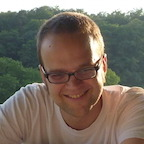
\includegraphics[width=\textwidth]{Thomas_Walter_Heidelberg.jpg}\\
\vspace{2em}
    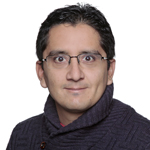
\includegraphics[width=\textwidth]{velascoforero}\\
\vspace{2em}
    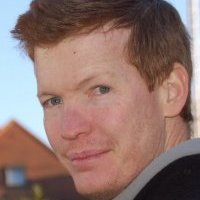
\includegraphics[width=\textwidth]{ed.jpg}

  \end{column}
  \begin{column}{.8\textwidth}

    \begin{block}{Thomas Walter \hfill \scriptsize{\url{http://members.cbio.mines-paristech.fr/\~twalter}}}
      \scriptsize{
    \begin{itemize}
    \item Researcher on bioimage informatics, director of CBIO
    \item Main application fields: High Content Screening, as a method to systematically study biological processes by analyzing cellular phenotypes
    \end{itemize}
    }
  \end{block}

  \begin{block}{Santiago Velasco-Forero  \hfill \scriptsize{\url{http://cmm.mines-paristech.fr/\~velasco}}}
      \scriptsize{
    \begin{itemize}
    \item Researcher on image processing, pattern recognition, multivariate statistics, graph-based data/image analysis
    \item Main application fields: Remote Sensing, cosmetology, astronomy, hyperspectral imaging.
    \end{itemize}
    }
  \end{block}

    \begin{block}{Etienne Decencière \hfill \scriptsize{\url{http://cmm.mines-paristech.fr/\~decenciere}}}
      \scriptsize{
    \begin{itemize}
    \item Researcher on image analysis, mathematical morphology, deep learning
    \item Main application fields: Ophthalmology, dermatology, cosmetology, astronomy
    \end{itemize}
    }
  \end{block}

  \end{column}
\end{columns}

}

%%%%%%%%%%%%%%%%%%%%%%%%%%%%%%%%%%%%
%% \begin{frame}{Teaching assistants}


%%       \begin{itemize}
%%         \item Monday: Arthur Imbert
%%       \item Tuesday: David Duque
%%       \item Wednesday: Leonardo Gigli
%%       \item Thursday: Bogdan Stanciulescu
%%       \item Friday: Tristan Lazard
%%       \end{itemize}

%% \end{frame}

%%%%%%%%%%%%%%%%%%%%%%%%%%%%%%%%%%%%
\begin{frame}{Course organization}

  \begin{itemize}
  \item During course sessions:
    \begin{itemize}
    \item Lectures
    \item Invited speakers
    \item Notebooks presentation and correction
    \end{itemize}
  \item Practical work (at home):
    \begin{itemize}
    \item Python
    \item keras, numpy
    \item Google colab
    \end{itemize}
  \item Communication
  \begin{itemize}
  \item General information available from: \url{http://cours.cmm.mines-paristech.fr}
  \item Forum (questions about the course and the notebooks): Slack
  \item E-mail (absence justification, etc.)
  \end{itemize}
\item Grading: written exam (march 17, 9am)
   \end{itemize}
\end{frame}


%%%%%%%%%%%%%%%%%%%%%%%%%%%%%%%%%%%%
\begin{frame}{Invited speakers}

  \begin{itemize}
  \item Vincent Morard (General Electric) : AI for medical images: an industrial point of view
    \item Bruno Figliuzzi (CMM, Mines Paris) : Segmentation d'images de rhéologie par réseaux de neurones convolutionnels
    \item Sébastien Lefèvre (IRISA) : DL and remote sensing
    \item Claire-Hélène Demarty (InterDigital) : Deep Learning for post production in movie industry
    \item Timothée Faucon (aiVision) : Deep learning for retinal image analysis
    \item Diego Tuccillo (Instituto de Astrofisica de Canarias): Deep learning applications in Astronomy
    \item Martin Bauw (CMM, Mines Paris): anomaly detection
    \item Valentin Penaud-Polge (CMM, Mines Paris): parametric layers
   \end{itemize}




\end{frame}


%% %%%%%%%%%%%%%%%%%%%%%%%%%%%%%%%%%%%%
%% \begin{frame}{Grading}

%% \begin{itemize}
%% \item Assignments
%% \item Exam
%% \end{itemize}

%% \end{frame}

%%%%%%%%%%%%%%%%%%%%%%%%%%%%%%%%%%%%
\begin{frame}{Main notations}
  \begin{eqnarray*}
    i, j, n, p, q & \hspace{1em} & \text{Integer scalars} \\
    x, y, z & \hspace{1em} & \text{Real scalars} \\
    \x, \y & \hspace{1em} & \text{Real vectors} \\
    \X, \W & \hspace{1em} & \text{Matrices} \\
    f, \act & \hspace{1em} & \text{Functions} \\
    \param & \hspace{1em} & \text{Set of parameters} \\
    \end{eqnarray*}
\end{frame}


%%%%%%%%%%%%%%%%%%%%%%%%%%%%%%%%%%%%
\begin{frame}{Bibliography}

  \begin{itemize}
  \item Ian Goodfellow and Yoshua Bengio and Aaron Courville, Deep learning, MIT Press. \url{https://www.deeplearningbook.org/}

  \item Trevor Hastie, Robert Tibshirani, Jerome Friedman, The elements of statistical learning, Springer. \url{https://web.stanford.edu/~hastie/ElemStatLearn/}

  \end{itemize}
\end{frame}



%% %%%%%%%%%%%%%%%%%%%%%%%%%%%%%%%%%%%%%%%%%%%%%%%%%%
%% \section*{References}

%% %%%%%%%%%%%%%%%%%%%%%%%%%%%%%%%%%%%%%%%%%%%%%%%%%%

%% \frame[allowframebreaks]{

%% \scriptsize

%% \frametitle{References}

%% %\bibliographystyle{amsalpha}
%% %\bibliographystyle{apalike}

%% \bibliography{edf.bib}

%% \normalsize

%% }

%%%%%%%%%%%%%%%%%%%%%%%%%%%%%%%%%%%%%%%%%%%%%%%%%%
%%%%%%%%%%%%%%%%%%%%%%%%%%%%%%%%%%%%%%%%%%%%%%%%%%
%%%%%%%%%%%%%%%%%%%%%%%%%%%%%%%%%%%%%%%%%%%%%%%%%%

\end{document}
